\begin{figure}
  \centering
  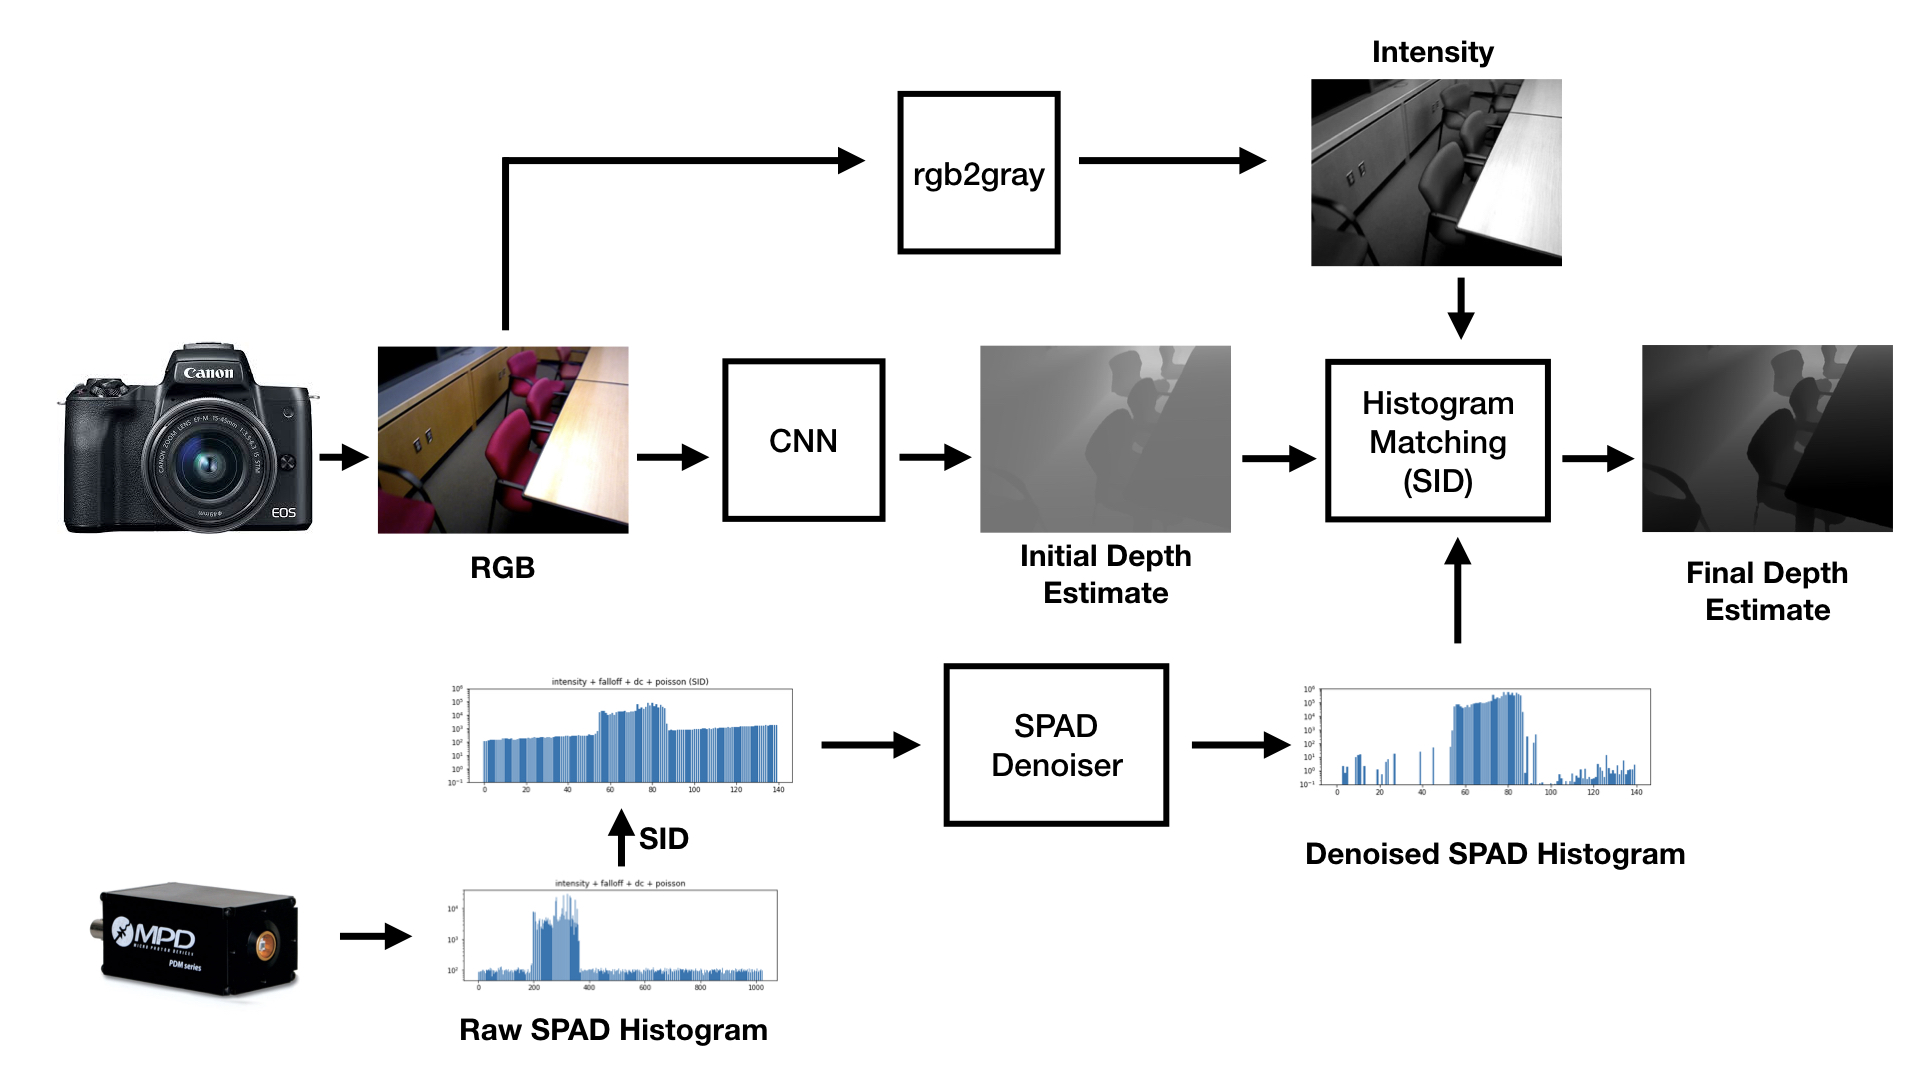
\includegraphics[width=\columnwidth]{full_pipeline.jpeg}
  \caption{\textbf{Overview of the full pipeline} We use a CNN to get an initial
  per-pixel depth estimate. Then we perform exact histogram matching using
  intensity-weighted pixel values on the corrected SPAD data.}
\end{figure}

Monocular depth estimation is a well-explored, yet active area of research (see Sec.~\ref{sec:related}). Any network trained for the MDE task takes as input an RGB image and estimates the depth map of the scene. Our approach augments existing MDE networks but is agnostic to the specific type of depth estimator. Indeed we show in Section~\ref{sec:evaluation} that our histogram matching technique equally improves a variety of different pre-trained estimators. In the remainder of this section, we therefore focus on modeling the image formation of a diffused single-photon avalanche diode (SPAD) and develop an approach to correcting an estimated depth map to match the global scene information captured by the SPAD.

%In this section, we describe the measurement model for a single-pixel time-of-flight lidar sensor under diffuse, pulsed laser illumination. 

%%%%%%%%%%%%%%%%%%%%%%%%%%%%%%%%%%%%%%%%%%%%%%%%%%%%%%%%%%%%%%%%%%%%%%%%%%%%%%%%%%%%%%%%%%%%%%%%%%%%%%%%%%%%%%%%%%%%
\subsection{Image Formation Model of a Diffused SPAD}

Consider a diffused laser that emits a pulse at time $t = 0$ with time-varying intensity $g(t)$ illuminating some 3D scene. We parameterize the geometry of the scene as a depth map $z(x, y)$, where each of the 3D points has also some unknown reflectivity $\alpha$ at the wavelength of the laser. Ignoring interreflections of the emitted light within the scene, a single-pixel diffused SPAD then integrates all the light scattered back from the scene towards the detector as
%
\begin{equation}
	s \left( t \right)= \int_{\Omega_x} \int_{\Omega_y} \frac{\alpha \left( x,y \right)}{z(x,y)^2}  g \left( t - \frac{2z(x,y)}{c} \right) dx dy ,
	\label{eq:pulse_integral} 
\end{equation}  
%
where $c$ is the speed of light and $\Omega_{x,y}$ is the angular range of the diffuser. In this formulation, we assume that the diffuser spreads light uniformly over all angles. Each time such a light pulse is emitted into the scene and scattered back to the detector, the single-pixel SPAD time-stamps up to one of the returning photons with some probability. This is not necessarily the first returning photon. The process is repeated millions of times per second with the specific number of emitted pulsed being controlled by the repetition rate of the laser, which is typically adjusted to match the deadtime of the SPAD~\cite{Heide:2018}. Each detected photon arrival event is discretized into a histogram $h$ of the form
%
\begin{equation}
  h[n] \sim \mathcal{P} \left( \eta \int_{n\Delta t}^{(n+1)\Delta t} \left(f * s \right) \left( t \right)  dt + b \right),	
	\label{eq:spad_measurements}
\end{equation}
%
where $(n\Delta t, (n+1) \Delta t)$ models the $n^{th}$ time interval of the
temporal histogram, $\eta$ is the photon detection probability of the SPAD, $f$
is a function that models the temporal uncertainty in the detector, and $b$
represents ambient background light and falsely detected photons known as dark
count. As derived in previous work, the combination of signal, background, and
noise can be modeled as an inhomogeneous Poisson process
$\mathcal{P}$~\cite{Kirmani:2014,Shin2015}. Finally, as in \cite{Xin2019} we adopt the term
\textit{transient} for our histogram $h[n]$.

\subsection{Ambient Rejection and Falloff Correction}
To remove the ambient and dark count photons from the histogram, we apply a
preprocessing step. Assuming that the first $N$ bins of the SPAD histogram
contain only ambient and dark count photons (this is equivalent to assuming the
minimum image depth is larger than $N \cdot c\Delta T/2$), we estimate 
and dark count rate $b$ as $\hat b = \frac{1}{N}\sum_{n=0}^N h[n]$ We then
note that that shining a laser through a 2D diffuser and
measuring a single pixel is very physically similar to recording a single 
non-line-of-sight measurement. We
compute the absolute first difference $d[n] = \abs{h[n] - h[n+1]}$ and find 
the set of edges. Intuitively, given a sufficiently large value of $b$, the Poisson sample
$h[n] \sim \mathcal{P}(b)$ should behave roughly like a Gaussian with variance $b$, and the difference
$h[n] - h[n+1]$ should behave like a Gaussian with variance $2b$. Therefore, we
can detect edges that occur between bins that contain actual signal photons and
bins that do not by computing the set 
\begin{equation}
  \mathcal{E} = \mset{n}{d[n] > \alpha\sqrt{2\hat b}}.
  \label{eq:edge_set}
\end{equation}
In this work, we use $\alpha = 2$.
We identify the closest and furthest edges $n_{first} = \min \mathcal{E}$ and
$n_{last} = \max \mathcal{E}$.
From \cite{Xin2019} Proposition 3, these edges
correspond to the discontinuties in the depth map 
at the closest and furthest image depths, and therefore all of the signal
photons must be in the bins between these two edges.
We refine these estimates by
computing $n'_{first} = \max\set{n_{first}}\cup\mset{n}{h[n] > \hat b, n \leq n_{first}}$ and
$n'_{last} = \min\set{n_{last}}\cup\mset{n}{h[n] > \hat b, n \geq n_{last}}$
Finally, we reject all photons outside of the valid range by clamping those bins
to 0, and we subtract our ambient estimate from the photons within the valid
range, giving an ambient-free transient
\begin{equation}
  h'_{clean}[n] = \begin{cases}
    0 & n < n'_{first} \\
    \max(h[n] - \hat b, 0) & n'_{first} \leq n \leq n'_{last} \\
    0 & n > n'_{last} \\
  \end{cases}.
  \label{eq:h_clean}
\end{equation}
To compensate for the radiometric falloff, we scale each bin by its squared depth,
which is consistent with our hardware prototype's radiometric falloff model.
This gives
\begin{equation}
  h_{clean}[n] = h'_{clean}[n] \cdot r_n^2
  \label{eq:h_scaled}
\end{equation}
where $r_n= \paren*{n + \frac12}\paren*{\frac{c\Delta t}{2}}$ is the depth
corresponding to bin $n$
As a final preprocessing step, we re-bin the transient, applying the Spacing-Increasing Discretization
(SID) of \cite{Fu2018} to produce $h_{target}$. This reduces the number of bins in the histogram
matching procedure, giving speedups while maintaining performance. In this work,
we use 140 bins for the simulated results and 600 bins for the captured results.

% \begin{itemize}
%   \item Talk about histogram matching in the ideal case, jump straight to intensity 
%   \item Talk about histogram matching in our case, and how it approaches the
%     ideal case. Discuss the following corrections 
%     \begin{itemize}
%       \item Ambient/DC - Use \cite{Xin2019} to justify looking for large edges,
%         then the ambient estimate to get rid of the noise floor.
%       \item Falloff
%     \end{itemize}
%   \item Talk about how the histogram matching works with intensity
%     considerations applied, briefly.
%   \item We don't address jitter or poisson noise.
% \end{itemize}
% \begin{equation}
%   h[n] \sim \mathcal{P}\paren*{\sum_{x,y}\alpha_{x,y}\eta \lambda_{x,y}[n] + b} \label{global_hints}
% \end{equation}
% Given a SPAD with histogram $h$ according to the above equation, we first
% process the SPAD to remove the effects of some of the terms. First, we 


%Neglecting albedo and falloff effects, an ideal detector counting photon events
%from a location $(x,y)$ in the time interval $(n\Delta t, (n+1) \Delta t)$ would record
%
%\begin{equation}
  %\lambda_{x,y}[n] = \int_{n\Delta t}^{(n+1) \Delta t} (f * g)\paren*{t - 2z(x,y)/c} dt \label{single_loc_spad} 
%\end{equation}  
%
%where $c$ is the speed of light, and $f$ is a function that models the temporal uncertainty in the
%detector. Single-photon avalanche diodes (SPADs) are highly sensitive
%photodetectors which are able to record single photon events with high temporal
%precision \cite{Stuff}. Since the event corresponding to the detection of a
%photon can be described with a Bernoulli random variable,
%the total number of accumulated photons in this time interval follows a Poisson
%distribution according to
%
%\begin{equation}
  %h[n] \sim \mathcal{P}\paren*{\sum_{x,y}\alpha_{x,y}\eta \lambda_{x,y}[n] + b} \label{global_hints}
%\end{equation}
%
%where $\alpha_{x,y} = r_{x,y}/z(x,y)^2$ captures the attenuation of the
%photon counts due to the reflectance $r(x,y)$ of the scene and due to the
%inverse square falloff $1/z(x,y)^2$.
%In addition, $\eta$ is the detection probability of a photon
%triggering a SPAD event, and $b = \eta a + d$ is the average number of background detections resulting
%from ambient photons $a$
%and erroneous ``dark count'' events $d$ resulting from noise within the SPAD.
%% \newpage
%% \begin{table*}[htbp]
%%   \begin{center}
  %%   \begin{tabularx}{\linewidth}{*{2}{X}}
  %%     \includegraphics[width=\textwidth/2-5pt]{sections/figures/spad_example/rgb.png} &
  %%     \includegraphics[width=\textwidth/2-5pt]{sections/figures/spad_example/rawdepth.png} \\
  %%     \includegraphics[width=\textwidth/2-5pt]{sections/figures/spad_example/depth_hist.png} &
  %%     \includegraphics[width=\textwidth/2-5pt]{sections/figures/spad_example/spad_hist.png} \\
  %%   \end{tabularx}
  %% \end{center}
  %% \caption{Sample Image. Top Left is the RGB image. Top Right is ground truth
  %%   depth. Bottom Left is Raw ground truth depth histogram. Bottom Right is
  %%   simulated SPAD measurements. Notice how closer depths are magnified and far
  %%   depths are attenuated.}
%% \end{table*}
%
%%%%%%%%%%%%%%%%%%%%%%%%%%%%%%%%%%%%%%%%%%%%%%%%%%%%%%%%%%%%%%%%%%%%%%%%%%%%%%%%%%%%%%%%%%%%%%%%%%%%%%%%%%%%%%%%%%%%
% \subsection{Monocular depth estimation with global depth hints}
% Given a single RGB image $I(x,y)$ and a vector of photon arrivals $h[n]$
% described by equation \ref{global_hints}, we seek to
% reconstruct the ground truth depth map $z(x,y)$.
% Our method has two parts. First, we \textbf{initialize} our estimate of the depth map from the single RGB
% image via a monocular depth estimator described below. Second, we \textbf{refine} this depth map using
% the captured measurements $h[n]$ via exact histogram matching. 

% \paragraph{Initialization}
% The first step in our method is to produce an initial estimate of ground truth
% depth. Convolutional Neural Networks have been shown to produce accurate, if poorly-scaled, estimates of depth
% from only a single image. We therefore choose to initialize our depth map
% estimate $\hat z^{(0)}(x,y)$ using
% a CNN. However, any depth estimator reliant on only a single
% view may be used for this step. Furthermore, in the larger context of our
% algorithm, it is more important that the network predict the correct ordinal
% relationships between pixels - that is, to predict the correct relative ordering
% of pixels $a$ and $b$, rather than to get all pixels exactly correct.

\subsection{Exact Histogram Matching}
% \begin{algorithm}[H]
%  \caption{Exact Histogram Matching} 
%  \label{alg:ehm}
%  \begin{algorithmic}[1]
  \Procedure{ExactHistogramMatching}{$I$, $W$, $t$}
  \State $s \gets \text{Histogram}(I, W)$
  \State $M \gets \text{zeros}(rows=\text{length(s)}, cols=\text{length}(t)))$ 
  \For{$i$ in $1,...,\text{length}(s)$}
    \For{$j$ in $1,...,\text{length}(j)$}
      \State $c_t \gets \sum_{\ell = 1}^{i-1} M_{\ell j}$
      \State $c_s \gets \sum_{\ell = 1}^{j-1} M_{i \ell}$
      \State $M_{ij} \gets \min(s_i - c_s, t_j - c_t)$
    \EndFor
  \EndFor
  \State $\hat I \gets \text{zeros}(\text{shape}(I))$
  \For{each pixel $p = I_{ij}$}
    \State $d = \frac{M_{p,:}}{\text{sum}(M_{p,:})}$ \Comment{$d$ is a
      probabilty distribution}
    \State Sample $q \in \set{1,...,length(t)}$ according to $d$.
    \State $\hat I_{ij} \gets q$
  \EndFor
  \State \textbf{return} $\hat I$
  \EndProcedure
\end{algorithmic}
  
% \end{algorithm}
Exact histogram matching is a procedure that takes a source image and a target
histogram and maps the pixel values of the source image so that the image's
histogram matches the target histogram. Given a single RGB image, we pass it
through an MDE to produce a depth map $\hat z_0 \in [\ell, u]^{M \times N}$
where $\ell$ and $u$ are the lower and upper bounds of the depth range of
interest, respectively. In a parallel processing step,
we compute an estimate of the scene albedo using an intrinsic imaging method and
take the color channel of the resulting albedo image that corresponds to the
wavelength of the laser illumination. This gives a reflectance estimate $W \in
[0, 1]^{M \times N}$. We
then compute a weighted histogram $h_{source}$of the depth map $\hat z_0$ where the
per-pixel weights are given by $W$, and the bin edges are given by the SID
discretization algorithm of \cite{Fu2018}.

We match the histogram $h_{source}$ to $h_{target}$ using the method of
\cite{Morovic2002}. We compute a pixel movement
matrix $T$ such that $T_{mn}$ is the amount of mass to move from $h_{source}[m]$
to $h_{target}$. We do so using the procedure outlined in \ref{alg:pixel_movement}

\begin{algorithm}[H]
 \caption{Pixel Movement} 
 \label{alg:ehm}
 \begin{algorithmic}
  \Procedure{FindMovement}{$h_s$ of length $M$, $h_t$ of length $N$} 
    \State Initialize $T$ as an $M \times N$ array.
    \For{$m$ in $1,\ldots,M$}
      \For{$n$ in $1,\ldots,N$}
        \State $p_s \gets \sum_{\ell=1}^{n-1} T[m, \ell]$
        \State $p_t \gets \sum_{\ell=1}^{m-1} T[\ell, n]$
        \State $T[m, n] \gets \min(h_s[m] - p_s, h_t[n] - p_t)$
      \EndFor
    \EndFor
    \State \textbf{return} $T$
  \EndProcedure
 \end{algorithmic}
\end{algorithm}

Finally, for a pixel $z_0[i, j]$ in depth bin $k$, we sample the new depth bin from the
distribution $T[k, :]/\sum_{n=1}^NT[k,n]$ (which is a distribution over target
depth bins $1,\ldots,N$) to get the bin of $\hat z[i,j]$. We can then apply the
standard SID decoding procedure to get the depth corresponding to that bin
\textcolor{red}{Does the above seem reasonable to include? Not sure if the
  pseudocode is helpful/necessary or not.}
%\subsection{Implementation Details}
%For the Monocular Depth Estimator, we use pretrained versions of the
%the Deep Ordinal Regression Network (DORN) \cite{} and the DenseDepth Network.
%The exact histogram matching method is as described in \cite{}.


